
\documentclass[11pt,a4paper]{article} %UKenglish,
\textheight24cm
\textwidth16cm
\topmargin-5mm
\oddsidemargin0cm
\evensidemargin0cm

\usepackage{enumerate}
\usepackage{textcomp}
\usepackage{url}
\usepackage{graphicx}
\usepackage[numbers]{natbib}
\usepackage{bussproofs}
\usepackage{tikz}
\usepackage{amssymb}
\usepackage{amsmath}
\usepackage{amsthm}
\usepackage{verbatim}
\usepackage{caption}
\usepackage{subcaption}
\usepackage[all,cmtip]{xy}
\usetikzlibrary{positioning, automata}
\usetikzlibrary{decorations.pathmorphing}
 \usetikzlibrary{snakes}
\usepackage[utf8]{inputenc}
\usepackage[russian]{babel}


\tikzset{snake it/.style={decorate, decoration=snake}}
\urlstyle{same}


\newcommand{\dftoutputlast}{\phi}

\newtheorem{lemma}{Lemma}
\newtheorem{theorem}{Theorem}
\newtheorem{definition}{Definition}
\newtheorem{example}{Example}
\newtheorem{corollary}{Corollary}


\begin{document}


\sloppy

\title{Rational index of bounded-oscillation languages\footnote{%
This research was supported by the Russian Science Foundation, project 18-11-00100.}}

\author{Ekaterina Shemetova\footnote{%
Department of Mathematics and Computer Science, St. Petersburg State University, 
7/9 Universitetskaya nab., Saint Petersburg 199034, Russia.}
\footnote{%
St. Petersburg Academic University, 
ul. Khlopina, 8, Saint Petersburg 194021, Russia.}
\footnote{%
JetBrains Research,
Primorskiy prospekt 68-70, Building 1, St. Petersburg, 197374, Russia.}
\and
Alexander Okhotin\footnotemark[2]
\and
Semyon Grigorev\footnotemark[2] \footnotemark[4]
}

\maketitle


\begin{abstract}
The rational index of a context-free language  $L$ is a function $f(n)$, such that for each regular language $R$ recognized by an automaton with $n$ states, the intersection of $L$ and $R$ is either empty or contains a word shorter than $f(n)$. It is known that the context-free language (CFL-)reachability problem and Datalog chain query evaluation for context-free languages (queries) with the polynomial rational index is in NC, while these problems is P-complete in the general case. We investigate the rational index of bounded-oscillation languages and show that it is of polynomial order. We obtain upper bounds on the values of the rational index for general bounded-oscillation languages and for some of its previously studied subclasses.

\textbf{Keywords.}
Bounded-oscillation languages; rational index; CFL-reachability; parallel complexity; context-free languages; Datalog programs; context-free path queries.
\end{abstract}


\section{Introduction}
\label{intro}
The notion of a rational index was introduced by Boasson et al. \cite{RatBasic} as a complexity measure for context-free languages. The rational index $\rho_L(n)$ is a function, which denotes the maximum length of the shortest word in $L \cap R$, for arbitrary $R$ recognized by an $n$-state automaton. The rational index plays an important role in determining the parallel complexity of such practical problems as the context-free language (CFL-)reachability problem and Datalog chain query evaluation.

The CFL-reachability problem for a fixed context-free grammar $G$ is stated as follows: given a directed edge-labeled graph $D$ and a pair of nodes  $u$ and $v$, determine whether there is a path from $u$ to $v$ labeled with a string in $L(G)$. That is, CFL-reachability is a kind of graph reachability problem with path constraints given by context-free languages. It is an important problem underlying some fundamental static code analysis like data flow analysis and program slicing \cite{RepsBasic}, alias analysis \cite*{Chatterjee, alias}, points-to analysis \cite{Incremental} and other \cite{Cai, android, typeflow}, and graph database query evaluation \cite{Azimov, GrigorevRagozina, HellingsCFPQ, RDF}. The \textit{Datalog chain query} evaluation on a database graph is equivalent to the CFL-reachability problem \cite{10.1145/28659.28685, Ullman}. 


Unlike context-free language recognition, which is in NC (when context-free grammar is fixed), the CFL-reachability problem is P-complete \cite{ PCompl, RepSeq,  Yannakakis}. Practically, it means that there is no efficient parallel algorithm for solving this problem (unless P $\neq$ NC). 


The question on the parallel complexity of Datalog chain queries was investigated independently \cite{ChainQ, Vardi, Ullman}. Ullman and Van Gelder \cite{Ullman} introduce the notion of a \textit{polynomial fringe property} and show that chain queries having this property is in NC. The polynomial fringe property is equivalent to having the polynomial rational index: for a context-free language $L(G)$ having the polynomial rational index $\rho_L(n) = poly(n)$, where $poly(n)$ is some polynomial, is the same as for corresponding chain query to have the polynomial fringe property. It has been shown that for every algebraic number $\gamma$, a language with the rational index in $\Theta (n^\gamma )$ exists \cite{GreibRat}.  In contrast, the rational index of languages, which generate all context-free languages (an example of such language is the Dyck language on two pairs of parentheses $D_2$) is in order $exp(\Theta(n^2/\ln n))$ \cite{CFRat}, and, hence, this is the upper bound on the value of the rational index for every context-free language.


While both problems is not parallelizable in general, it is useful to develop more efficient parallel solutions for specific subclasses of the context-free languages. For example, there are context-free languages which admit more efficient parallel algorithms in comparison with the general case of context-free recognition \cite{IBARRA2, IBARRA, Okhotin2014ComplexityOI}.  The same holds for the CFL-reachability problem: there are some examples of context-free languages, for which the CFL-reachability problem lies in NL complexity class (for example, linear and one-counter languages) \cite{labelledGraphs, LReach, Regularrealizability, VyalyiRR}. These languages have the polynomial rational index.


The family of linear languages (linear Datalog chain programs, respectively) is the well-known subclass of context-free languages having the polynomial rational index \cite{RatBasic, Ullman}. The value of its rational index is in $O(n^2)$ \cite{RatBasic}. It is known that problems solvable by a linear Datalog Program are solvable in non-deterministic logarithmic space and, hence,  highly parallelizable. This class has received a lot of interest in complexity of constraint satisfaction, deductive databases and logic \cite{ linearisability, Dalmau2005LinearDA, linopt, Ullman}. 





In this work we investigate the rational index of  bounded-oscillation languages. Bounded-oscillation languages were introduced by Ganty and Valput \cite{BoundOsc} as the generalization of the class of linear languages. Just like linear languages, it is defined by restriction on the pushdown automata. This restriction is based on the notion of \textit{oscillation}, a special measure of how the stack height varies over time. 


\textbf{Our contributions.} Our results can be summarized as follows:
\begin{itemize}
\item We show that the rational index of bounded-oscillation languages of Ganty and Valput \cite{BoundOsc} is polynomial and give an upper bound on its value in dependence of the value of oscillation.
\item We give upper bounds on the value of rational indices of previously studied subclasses of bounded-oscillation languages: superlinear and ultralinear languages.
\end{itemize}





\section{Preliminaries}
\label{sec:prel}
\label{preliminaries}
\paragraph{Formal languages.} 
A \textit{context-free grammar} is a 4-tuple $G = (\Sigma, N, P, S)$, where $\Sigma$ is a finite set of alphabet symbols,  $N$ is a set of nonterminal symbols, $P$ is a set of production rules and $S$ is a start nonterinal. $L(G)$ is a context-free language generated by context-free grammar $G$. We use the notation $A \stackrel {*}{\Rightarrow } w$  to denote that the string $w \in \Sigma^*$ can be derived from a nonterminal $A$ by sequence of applying the production rules from $P$. A \textit{parse tree} is an entity which represents the structure of the derivation of a terminal string from some nonterminal.


A grammar $G$ is said to be is in the \textit{Chomsky normal form}, if all production rules of $P$ are of the form:
$A \rightarrow BC$, $A \rightarrow a$ or $S \rightarrow \varepsilon$, where $A, B, C \in N$ and $a \in \Sigma$. 


The set of all context-free languages is identical to the set of languages accepted by pushdown automata (PDA). \textit{Pushdown automaton} is a 7-tuple $M = (Q, \Sigma, \Gamma, \delta, q_0, Z, F)$, where $Q$ is a finite set of states, $\Sigma$ is a input alphabet, $\Gamma$ is a finite set which is called the stack alphabet, $\delta$ is a finite subset of $Q \times (\Sigma \cap \{\varepsilon\}) \times \Gamma \times Q \times \Gamma^*$,
$q_{0}\in Q$ is the start state, $Z \in \Gamma$ is the initial stack symbol and
$F\subseteq Q$ is the set of accepting states.


A \textit{regular language} is a language that can be expressed with a regular expression or a deterministic or non-deterministic finite automata.
A \textit{nondeterministic finite automaton} (NFA) is represented by a 5-tuple, $(Q,\Sigma ,\delta ,Q_{0},F)$, where $Q$ is a finite set of states, $\Sigma$ is a finite set of input symbols, $\delta:Q\times \Sigma \rightarrow 2^{|Q|}$ is a transition function, $Q_0 \subseteq Q$ is a set of initial states, $F \subseteq Q$ is a set of accepting (final) states. \textit{Deterministic finite automaton} is a NFA with the following restrictions: each of its transitions is uniquely determined by its source state and input symbol, and reading an input symbol is required for each state transition.


 For a language $L$ over an alphabet $\Sigma$, its rational index $\rho_L$ is a function defined as follows:
$$\rho_L(n) = \max_{\mathcal{A} \text{:NFA with }n\text{ states}, L \cap L(\mathcal{A}) \neq \emptyset}\ \min_{w \in  L \cap L(\mathcal{A})}|w|.$$ 

\paragraph{Languages of bounded dimension.} 
For each node $v$ in a tree $t$, its dimension $dim(v)$ is inductively defined as follows:
\begin{itemize}
\item if $v$ is a leaf, then $dim(v)$ = 0
\item if $v$ is an internal node with $k$ children $v_1, v_2, ..., v_k$ for $k \ge 1$, then 
$$
dim(v) = 
 \begin{cases}
   \max_{i \in \{1...k\}}dim(v_i) &\text{if there is a unique maximum}\\
   \max_{i \in \{1...k\}}dim(v_i)+1 &\text{otherwise}
 \end{cases}
$$
\end{itemize}


The dimension of a parse tree $t$ $dim(t)$ is the dimension of its root. 
It is observable from the definition that the dimension of a tree $t$
is the height of the largest perfect binary tree,
which can be obtained from $t$ by contracting edges and accordingly identifying vertices.
A tree of dimension $dim(t) = 2$ is illustrated in Figure~\ref{oscbtree}.
\begin{figure}
\centering
\begin{tikzpicture}[
level 1/.style={sibling distance=3cm},
level 2/.style={sibling distance=1.5cm}]
%\tikzstyle{every node}=[circle,draw]

\node[circle,draw] (Root) [ fill=red, red] {}
    child {
    node[circle,draw, blue] (l) {} 
    child { node[circle,draw, fill=red, red](ll) {}
            child { node[circle,draw, blue] (p) {} }
            child { node[circle,draw, blue] (pl) {} }
             }
    child { node[circle,draw, blue](lr) {} 
          child { node[circle,draw, blue] (plr) {} }
      }
}
child {
    node[circle,draw,  fill=red, red] (r) {}
    child { node[circle,draw, blue] (rl) {}} 
    child { node[circle,draw, blue] (rr) {} }
};
\node  [right=0.05cm of p] {0};
\node  [right=0.1cm of Root] {$2, dim(t)=2$};
\node  [right=0.05cm of l] {1};
\node  [right=0.05cm of r] {1};
\node  [right=0.05cm of ll] {1};
\node  [right=0.05cm of lr] {0};
\node  [right=0.05cm of pl] {0};
\node  [right=0.05cm of plr] {0};
\node  [right=0.05cm of rl] {0};
\node  [right=0.05cm of rr] {0};
\end{tikzpicture}
\caption{A tree $t$ with $dim(t)=2$. Nodes having children without unique maximum are filled.}
\label{oscbtree}            
\end{figure}

\begin{definition}[Grammars of bounded dimension]
Context-free grammar $G$ is of bounded dimension if the every parse tree $t$ of $G$ has $dim(t) \le d$, where $d$ is some constant. Then $d$ is called a dimension $dim(G)$ of $G$.
\end{definition}

\begin{definition}[Languages of bounded dimension]
Languages of bounded dimension are languages generated by grammars of bounded dimension. 
\end{definition}







\paragraph{Bounded-oscillation languages.} 
Oscillation is defined using a hierarchy of \textit{harmonics}. Let $\bar{a}$ be a \textit{push}-move and $a$ be a \textit{pop}-move. Then a PDA run $r$ can be described by a well-nested sequence $\alpha(r)$ of $\bar{a}$-s and $a$-s. Two positions $i<j$ form a \textit{matching pair} if the corresponding $\bar{a}$ at $i$-th position of the sequence matches with $a$ at $j$-th position. For example, word $\bar{a}\bar{a}\bar{a}aa\bar{a}aa$ has the following set of matching pairs: $\{(1, 8), (2, 5), (3, 4), (6, 7)\}$ ($\bar{a}(\bar{a}(\bar{a}a)a)(\bar{a}a)a$).


Harmonics are inductively defined as follows:
\begin{itemize}
\item  order 0 harmonic $h_0$ is $\varepsilon$
\item  $h_{(i+1)}$ harmonic is $\bar{a}h_ia\ \bar{a}h_ia$.
\end{itemize}
\begin{figure}
\centering
\begin{tikzpicture}
    \draw[thick, dashed, opacity=0.3] (0,0.5) -- (6,0.5);
     \draw[thick, dashed, opacity=0.3] (0,1) -- (6,1);
      \draw[thick, dashed, opacity=0.3] (0,1.5) -- (6,1.5);
      \draw[->] (0,0) -- (6,0) node[right] {step};
      \draw[->] (0,0) -- (0,2) node[above] {stack height};
     \draw[->, blue] (0,0) -- (0.5,0.5);
      \draw[->, blue] (0.5,0.5) -- (1,1);
      \draw[->, blue] (1,1) -- (1.5,1.5);
       \draw[->, orange] (1.5,1.5) -- (2,1);
    \draw[->, orange] (2,1) -- (2.5,0.5);
    \draw[->, blue] (2.5,0.5) -- (3,1);
    \draw[->, orange] (3,1) -- (3.5,0.5);
 \draw[->, orange] (3.5,0.5) -- (4,0);
\node (null) at (-0.1, 0) {0}; 
\node (one) at (-0.1, 0.5) {1}; 
\node (two) at (-0.1, 1) {2}; 
\node (three) at (-0.1, 1.5) {3}; 
    \end{tikzpicture}
\caption{Stack heights during the run of PDA.}
\label{oscb}
\end{figure}


PDA run $r$ is \textit{k-oscillating} if the harmonic of order $k$ is the greatest harmonic that occurs in $r$ after removing $0$ or more matching pairs. 

\begin{definition}[Bounded-oscillation languages]
Bounded-oscillation languages are languages accepted by pushdown automata with all runs $k$-oscillating. 
\end{definition}
It is important that the problem whether a given CFL is a bounded-oscillation language is undecidable \cite{BoundOsc}.

\begin{example}
Consider Figure \ref{oscb}. It shows how the stack height changes during the run of a PDA. Corresponding well-nested word $\alpha(r)$ is $\bar{a}\bar{a}\bar{a}aa\bar{a}aa$. The greatest harmonic in this word is order 1 harmonic (moves forming harmonic are marked in bold, removed matching pairs are $(1, 8)$ and $(2, 5)$): $\bar{a}\bar{a}\mathbf{\bar{a}a}a\mathbf{\bar{a}a}a$, therefore oscillation of the run $r$ is 1.
\end{example}


The oscillation of a parse tree of a context-free grammar can be defined similarly to the oscillation of a PDA run. Given a parse tree $t$, we define corresponding well-nested word $\alpha(t)$ inductively as follows:
\begin{itemize}
\item if $n$ is the root of $t$ then $\alpha(t) = \bar{a}\alpha(n)$
\item if $n$ is a leaf then $\alpha(n)=a$
\item if $n$ has $k$ children then $\alpha(n) = a\underbrace{\bar{a}...\bar{a}}_\text{$k$ times}\alpha(n_1)...\alpha(n_k)$
\end{itemize}


Moreover, given a PDA run $r$, there exists a corresponding parse tree $t$ with the same well-nested word $\alpha(t)=\alpha(r)$ and vice versa \cite{BoundOsc}. Therefore, a language $L$ is of bounded oscillation if all parse trees in a corresponding context-free grammar have bounded oscillation.


The oscillation of a parse tree is closely related with its dimension. 
It is known that the dimension of parse trees and its oscillation are in linear relationship.

\begin{lemma}[\cite{BoundOsc}]
\label{boscdim}
Let a grammar $G = (\Sigma, N, P, S)$ be in Chomsky normal form and let $t$ be a parse tree of $G$. Then $osc(t) - 1 \le dim(t) \le 2osc(t)$.
\end{lemma}
Thus if language $L$ is bounded-oscillation language then all parse trees in a corresponding context-free grammar have bounded dimension.
\paragraph{Context-free language reachability.} 
A \textit{directed labeled graph} is a triple $D = (Q, \Sigma, \delta)$, where $Q$ is a finite set of nodes, $\Sigma$ is a finite set of alphabet symbols,
and $\delta \subseteq Q \times \Sigma \times Q$ is a finite set of labeled edges. Let $L(D)$ denote a graph language a regular language, which is recognized by the NFA $(Q,\Sigma ,\delta ,Q, Q)$ obtained from $D$ by setting every state as inial and accepting.


Let $i\pi j$ denote a unique path between nodes $i$ and $j$ of the input graph and $l(\pi)$ denote a unique string obtained by concatenating edge labels along the path $\pi$. Then the CFL-reachability can be defined as follows.
\begin{definition}[Context-free language reachability]
Let $L \subseteq \Sigma^*$ be a context-free language and $D = (Q, \Sigma, \delta)$ be a directed labeled graph. Given two nodes $i$ and $j$ we say that $j$ is \textit{reachable} from $i$ if there exists a path $i \pi j$, such that $l(\pi) \in L$. 
\end{definition}
There are four varieties of CFL-reachability problems: all-pairs problem, single-source problem, single-target problem and single-source/single-target problem \cite{RepsBasic}. In this paper we consider single-source/single-target problem. 



\section{Rational index of languages of bounded dimension}
\label{sec:osc}
\subsection{Upper bounds on the rational index of languages of bounded dimension}
Before we consider the value of the rational index for languages of bounded dimension, we need to prove the following.
\begin{lemma}
\label{lem:treeheight}
Let  $G = (\Sigma, N, P, S)$ be a context-free grammar in Chomsky normal form,  $D=(V, E, \Sigma)$ be a directed labeled graph with $n$ nodes. Let $w$ be the shortest string in $L(G)\cap L(D)$. Then the height of every parse tree for $w$ in $G$ does not exceed $|N|n^2$.
\end{lemma}

\begin{proof}
Consider grammar $G'$ for $L(G)\cap L(D)$. The grammar $G = (\Sigma, N', P', S')$ can be constructed from $G$ using the classical construction by Bar-Hillel et al.~\cite{BarHillel}: $N' \subseteq N \times V \times V $  contains all tiples $(A, i, j)$ such that $A \in N, i, j \in V$ ; $P'$ contains production rules in one of the following forms:
\begin{enumerate}
\item $(A, i, j) \rightarrow (B, i, k), (C, k, j)$ for all $(i, k, j)$ in $V$  if $A \rightarrow BC \in P$
\item $(A, i, j) \rightarrow a$ for all $(i, j)$ in $V$ if $A \rightarrow a$.
\end{enumerate}
A triple $(A, i, j)$ is \textit{realizable} if and only if there is a path $i\pi j$ such that $A \stackrel {*}{\Rightarrow } l(\pi)$ for some nontermimal $A \in N$. Then the parse tree $t_G$ for $w$ in $G$ can be converted into parse tree $t_{G'}$ in $G'$. Notice that every node of $t_{G'}$ is realizable triple. Also it is easy to see that the height of $t_G$ is equal to the height of $t_{G'}$. Assume that $t_{G'}$ for $w$ has a height of more than $|N|n^2$. Consider a path from the root of the parse tree to a leaf, which has length greater than $|N|n^2$. There are $|N|n^2$ unique labels $(A, i, j)$ for nodes of the parse tree, so according to the pigeonhole principle, this path has at least two nodes with the same label. This means that the parse tree for $w$ contains at least one subtree $t$ with label $(A, i, j)$ at the root, which has a subtree $t'$ with the same label. Then we can change $t$ with $t'$ and get a new string $w'$ which is shorter than $w$, because the grammar is in Chomsky normal form. But $w$ is the shortest, then we have a contradiction.
\end{proof}
From Lemma~\ref{lem:treeheight} one can deduce an alternative proof of the fact that the rational index of linear languages is in $O(n^2)$ \cite{RatBasic}: the number of leaves in a parse tree in linear grammar in Chomsky normal form is proportional to its height, and thus it is in $O(n^2)$.
\begin{theorem}
\label{oscbnddim}
Let $G = (\Sigma, N, P, S)$ be a grammar of bounded dimension $dim(G) = d$ in Chomsky normal form, where $d$ is some constant. Let $D$ be a directed labeled graph with $n$ nodes. Then $\rho_{L(G)}$ is in $O(n^{2d})$ in the worst case.
\end{theorem}
\begin{proof}
Proof by induction on $dim(G)$.

\textbf{Basis.} $dim(G) = 1$.
\\
Рассмотрим дерево разбора $t$ в грамматике $G$. Размерность грамматики $G$ $dim(G) = 1$, следовательно размерность дерева $t$ (и его корня) не превысит $1$. Так как грамматика в нормальной форме Хомского, корень $t$ имеет двоих детей. По определению размерности, возможны 2 варианта значений размерности для детей:
\begin{enumerate}
\item Оба ребёнка имеют размерность 0 (являются листьями), тогда строка, порождаемая $t$, имеет длину 2.
\item Один из детей имеет размерность 0 (лист), второй имеет размерность 1. Тогда $t$ можно рекурсивно построить как дерево, на каждом уровне (кроме последнего), имеющее один лист и одну вершину размерности 1.  По Лемме ~\ref{lem:treeheight} высота $t$ не превышает $O(n^2)$, следовательно максимальное число листьев в $t$, и соответственно, $\rho_{L(G)}$ не превышает $O(n^2)$. 
\end{enumerate}
\textbf{Inductive step.} $dim(G) = d$.
\\
Рассмотрим дерево разбора $t$ в грамматике $G$. Пусть $S \rightarrow AB \in P$. Снова рассмотрим детей корня $t$. Корень $t$ помечен нетерминалом $S$, а его дети помечены нетерминалами $A$ и $B$ соответственно. Пусть $G(A)$ --- грамматика, полученная заменой в $G$ стартового нетерминала на $A$ ($G(A) \subset G$), а $G(B)$ --- заменой стартового нетерминала на $B$.  Рассмотрим возможные размерности $G(A)$ и $G(B)$. По определению размерности, возможны 2 случая:
\begin{enumerate}
\item $dim(G(A)) = dim(G(B)) = d-1$. Тогда, по индукционному предположению, длина слова, генерируемого $G(A)$ и $G(B)$, не превышает $O(n^{2(d-1)})$, тогда длина слова, генерируемого $t$ не превысит $O(n^{2(d-1)} + n^{2(d-1)}) = O(n^{2(d-1)})$.
\item $dim(G(A)) < d$ и $dim(G(B)) = d$. Пусть $dim(G(A)) = d - 1$. Тогда $t$ можно рекурсивно построить как дерево, на каждом уровне которого есть вершина с размерностью $d-1$, помеченная нетерминалом $X$, таким, что $dim(G(X)) = d - 1$, и вершина размерностью $d$. По Лемме ~\ref{lem:treeheight} высота $t$ не превышает $O(n^2)$, а по индукционному предположению длина слова, порождаемого $G(X)$ c $dim(G(X)) = d - 1$ не превышает $O(n^{2(d-1)})$. Тогда максимальная длина слова, порождаемого $t$, не превысит $O(n^2)O(n^{2(d-1)}) = O(n^{2d})$.

Случай $dim(G(A)) = d$ и $dim(G(B)) < d$ доказывается симметрично.
\end{enumerate}
\end{proof}
Комбинируя Теорему~\ref{oscbnddim} и Лемму~\ref{boscdim}, получаем следующее следствие.
\begin{corollary}
Let $L$ be a $k$-bounded-oscillation language. Then $\rho_{L(G)}$ does not exceed $O(n^{4k})$.
\end{corollary}

\begin{figure}
\centering
\begin{subfigure}{.5\textwidth}
  \centering
\begin{tikzpicture}[
level 1/.style={sibling distance=3cm},
level 2/.style={sibling distance=1.5cm}]
%\tikzstyle{every node}=[circle,draw]

\node[circle,draw] (Root) [ ] {$S$}
    child {
    node[circle,draw] (l) {$A$} 
}
    child {
    node[circle,draw] (r) {$B$} 
};
\node  [right=0.1cm of Root] {$d, dim(t)=d$};
\node  [right=0.05cm of l] {$d-1$};
\node  [right=0.05cm of r] {$d-1$};
\end{tikzpicture}
  \caption{$dim(G(A)) = dim(G(B)) = d-1$}
  \label{dimupper:1}
\end{subfigure}%
\begin{subfigure}{.5\textwidth}
  \centering
\begin{tikzpicture}[
level 1/.style={sibling distance=3cm},
level 2/.style={sibling distance=1.5cm}]
%\tikzstyle{every node}=[circle,draw]

\node[circle,draw, blue] (Root) [ ] {$S$}
    child {
    node[circle,draw] (l) {${A}$}  
}
child {
    node[circle,draw, blue] (r) {$B$}
    child { node[circle,draw, blue] (rl) {$Y$}     child {
    node[circle,draw] (rlr) {$X$}  
}
child {
    node[circle,draw, blue] (rll) {$B$}  
}
} 
    child { node[circle,draw] (rr) {$X$}  }
};
\node  [right=0.1cm of Root] {$d, dim(t)=d$};
\node  [right=0.05cm of l] {$d-1$};
\node  [right=0.05cm of r] {$d$};
\node  [left=0.02cm of rl] {$d$};
\node  [right=0.02cm of rr] {$d-1$};
\node  [left=0.05cm of rlr] {$d-1$};
\node  [right=0.02cm of rll] {$d$};
\end{tikzpicture}
  \caption{$dim(G(A)) = d-1$ и $dim(G(B)) = d$}
  \label{dimupper:2}
\end{subfigure}
\caption{Два варианта для размерностей детей корня дерева}
\label{dimupper}
\end{figure}

\label{sec:osc_lower}
\subsection{Lower bounds on the rational index of languages of bounded dimension}
\begin{theorem} Let $G$ be a grammar of bounded dimension $dim(G) = d$, where $d$ is some constant. Then there exists a language $L(G)$ with rational index in $O(n^{2d})$ for any $n$.
\begin{proof} Будем строить граф и грамматику для худшего случая индуктивно по $dim(G)$.

\textbf{База.} $dim(G) = 1$.
Языки, обладающие размерностью $d = 1$ совпадают с семейством линейных языков. Рассмотрим линейную грамматику $G_1=(\{a, b\}, \{A, B, S, S_1\}, \{S \rightarrow AB\ |\ AS_1, S_1 \rightarrow SB, A \rightarrow a, B \rightarrow b\}, S)$, порождающую язык $L(G_1) = \{a^kb^k \vert k > 0\}$. Рассмотрим NFA $\mathcal{A}_1$, состоящий из двух циклов взаимно простой длины ($m$ и $m'$ соответственно), имеющих одну точку сочленения (рисунок~\ref{worstd_1}). Пусть рёбра первого цикла помечены символом $a$, а второго символом $b$.  Зафиксирум состояние $q_0$, соответствующее точке сочленения, как финальное и стартовое. Тогда кратчайшая длина слова $l(q_0\pi q_0) \in L(G_1) \cap L(\mathcal{A}_1)$ не превысит $2mm'$. Пусть в автомате $\mathcal{A}_1$ $n$ состояний, тогда возьмем $m' = n/2$, $m = n/2 + 1$. Очевидно, что $m$ взаимно просто с $m'$. Тогда $l(q_0\pi q_0) \in L(G_1) \cap L(\mathcal{A}_1) = 2mm' = 2n/2(n/2 + 1) = O(n^2) = O(n^{2d})$. Данный пример хорошо известен сообществу \cite{HellingsCFPQ, Yannakakis}. 


\begin{figure}[h]
    \centering        
    \begin{tikzpicture}[shorten >=1pt,auto]
       \node[state] (q_0)                      {$q_1$};
       \node[state] (q_1) [above right=of q_0] {$q_2$};
       \node[state,  initial below, accepting] (q_2) [right=of q_0]       {$q_0$};
       \node[state] (q_3) [right=of q_2]       {$q_3$};
        \path[->]
        (q_0) edge  node {a} (q_1)
        (q_1) edge   node {a} (q_2)
        (q_2) edge  node {a} (q_0)
        (q_2) edge[bend left, above]  node {b} (q_3)
        (q_3) edge[bend left, below]  node {b} (q_2);
    \end{tikzpicture}

\caption{Worst-case NFA $\mathcal{A}_1$ for $L(G_1)$ and $n=4$ ($m = 3, m' = 2$). }
\label{worstd_1}
\end{figure}

\textbf{Индукционный переход.} $dim(G) = d$.
Пусть даны грамматика $G_{d-1} =  (\Sigma_{d-1}, N_{d-1}, P_{d-1}, S_{d-1})$ в нормальной форме Хомского с размерностью $dim(G_{d-1}) = d-1$, NFA $\mathcal{A}_{d-1}= (Q_{d-1},\Sigma_{d-1} ,\delta_{d-1} ,q^{d-1}_{0},\{q^{d-1}_{0}\})$ на $n'$ вершинах. Пусть $w_0^{d-1}$ --- кратчайшая строка в языке $L(G_{d-1}) \cap L(\mathcal{A}_{d-1})$.


\textit{Построение грамматики $G_d = (\Sigma_{d}, N_{d}, P_{d}, S_{d})$}. Грамматика $G_d$ задается следующим образом:
\begin{itemize}
\item $\Sigma_{d} = \Sigma_{d-1} \cup \{a_d, b_d, c_d\}$
\item $P_{d} = P_{d-1} \cup P'$, where $P' = 
\{ 
\\ S_d \rightarrow A_dS'_d\ \vert \ A_d\widehat{C}_d,
\\ S'_d \rightarrow S_d\widehat{C}_d,
\\A_d \rightarrow \widehat{A}_dA'_d,
\\A'_d \rightarrow A_d\widehat{B}_d \ \vert \ S_{d-1} \widehat{B}_d,
\\ \widehat{A}_d \rightarrow a_d,
\\ \widehat{B}_d \rightarrow b_d,
\\ \widehat{C}_d \rightarrow c_d
 \}$. 
\\ Заметим, что $P'$ соответствует множеству правил $\{  S_d \rightarrow A_dS_dc_d\vert A_dc_d; A_d \rightarrow a_dA_db_d \vert  a_dS_{d-1}b_d\}$, представленных в нормальной форме Хомского.
\item $N_d = N_{d-1} \cup \{S_d, A_d, S'_d, A'_d, \widehat{A}_d, \widehat{B}_d, \widehat{C}_d\}$. 

\end{itemize}
Покажем, что размерность $dim(G_d) = dim(G_{d-1}) + 1 = d$. Присвоим каждому нетерминалу $X \in N_d$ максимально возможную размерность $dim(X)$ вершины дерева разбора, помеченной данным нетерминалом. По условию $dim(S_{d-1}) = d-1$.
Рассмотрим дерево для следующего вывода $A_d \Rightarrow \widehat{A}_dA'_d \Rightarrow a_dA'_d \Rightarrow a_dS_{d-1} \widehat{B}_d \Rightarrow a_dS_{d-1} b_d$ (рисунок~\ref{dimsubtree:1}).  Нетрудно заметить, что для данного дерева $dim(A_d) = dim(S_{d-1}) = d-1$. Многократное применение правил $A_d \rightarrow \widehat{A}_dA'_d$ и $A'_d \rightarrow A_d\widehat{B}_d$ не меняет данного соотношения, так как они подвешивают только листья, размерность которых $0 < d - 1$. 


Рассмотрим дерево для вывода 
$S_d  \Rightarrow A_d S'_d \Rightarrow A_d S_d \widehat{C}_d \Rightarrow A_d A_d \widehat{C}_d \widehat{C}_d$ (рисунок~\ref{dimsubtree:2}). Идем по дереву снизу-вверх. Размерность $dim(A_d) = d - 1$, применение правила $S_d \rightarrow  A_d\widehat{C}_d$ оставляет размерность соответствующей вершины, помеченной $S_d$, равной $d-1$, так как второй ребенок этой вершины является родителем листа и имеет размерность $0$. То же самое происходит при применении правила $S'_d \rightarrow S_d\widehat{C}_d$, размерность вершины, помеченной $S'_d$ остается равной $d-1$. А вот применение правила $S_d \rightarrow A_dS'_d$ увеличивает размерность корня рассматриваемого дерева и делает ее равной $d-1+1 = d$, т.к. оба ребёнка корня имеют размерность $d-1$. Заметим, что дальнейшее применение правил (подвешивание поддеревьев) $S_d \rightarrow A_dS'_d$ и $S'_d \rightarrow S_d\widehat{C}_d$ не увеличит значение размерности: у вершины, помеченной $S_d$ всегда будет 2 ребёнка --- первый, помеченный нетерминалом $A_d$ с максимальной размерностью $d-1$ и второй, помеченный нетерминалом $S'_d$ с максимальной размерностью $d$. Таким образом, размерность корня дерева разбора $G_d$ не превысит $d$.

\begin{figure}
\centering
\begin{subfigure}{.5\textwidth}
  \centering
\begin{tikzpicture}[
level 1/.style={sibling distance=3cm},
level 2/.style={sibling distance=1.5cm}]
%\tikzstyle{every node}=[circle,draw]

\node[circle,draw] (Root) [ ] {$A_d$}
    child {
    node[circle,draw] (l) {$\widehat{A}_d$} 
    child { node[circle,draw](ll) {$a_d$}
             }
}
child {
    node[circle,draw] (r) {$A'_d$}
    child { node[circle,draw] (rl) {$S_{d-1}$}} 
    child { node[circle,draw] (rr) {$\widehat{B}_d$} child { node[circle,draw](rr0) {$b_d$}
             } }
};
\node  [right=0.1cm of Root] {$d-1, dim(t)=d-1$};
\node  [right=0.05cm of l] {0};
\node  [right=0.05cm of r] {$d-1$};
\node  [right=0.05cm of ll] {0};
\node  [below=0.02cm of rl] {$d-1$};
\node  [right=0.02cm of rr] {0};
\node  [right=0.02cm of rr0] {0};
\end{tikzpicture}
  \caption{Дерево разбора для $A_d$}
  \label{dimsubtree:1}
\end{subfigure}%
\begin{subfigure}{.5\textwidth}
  \centering
\begin{tikzpicture}[
level 1/.style={sibling distance=3cm},
level 2/.style={sibling distance=1.5cm}]
%\tikzstyle{every node}=[circle,draw]

\node[circle,draw] (Root) [ ] {$S_d$}
    child {
    node[circle,draw] (l) {${A}_d$}  
}
child {
    node[circle,draw] (r) {$S'_d$}
    child { node[circle,draw] (rl) {$S_{d}$}     child {
    node[circle,draw] (rlr) {${A}_d$}  
}
child {
    node[circle,draw] (rll) {$\widehat{C}_d$}  
}
} 
    child { node[circle,draw] (rr) {$\widehat{C}_d$}  }
};
\node  [right=0.1cm of Root] {$d, dim(t)=d$};
\node  [right=0.05cm of l] {$d-1$};
\node  [right=0.05cm of r] {$d-1$};
\node  [left=0.02cm of rl] {$d-1$};
\node  [right=0.02cm of rr] {0};
\node  [left=0.05cm of rlr] {$d-1$};
\node  [right=0.02cm of rll] {$0$};
\end{tikzpicture}
  \caption{Дерево разбора для $S_d$}
  \label{dimsubtree:2}
\end{subfigure}
\caption{Поддеревья разбора для $G_d$ и размерности их вершин}
\label{dimsubtree}
\end{figure}


\begin{figure}
\centering
\begin{minipage}{.5\textwidth}
  \centering
  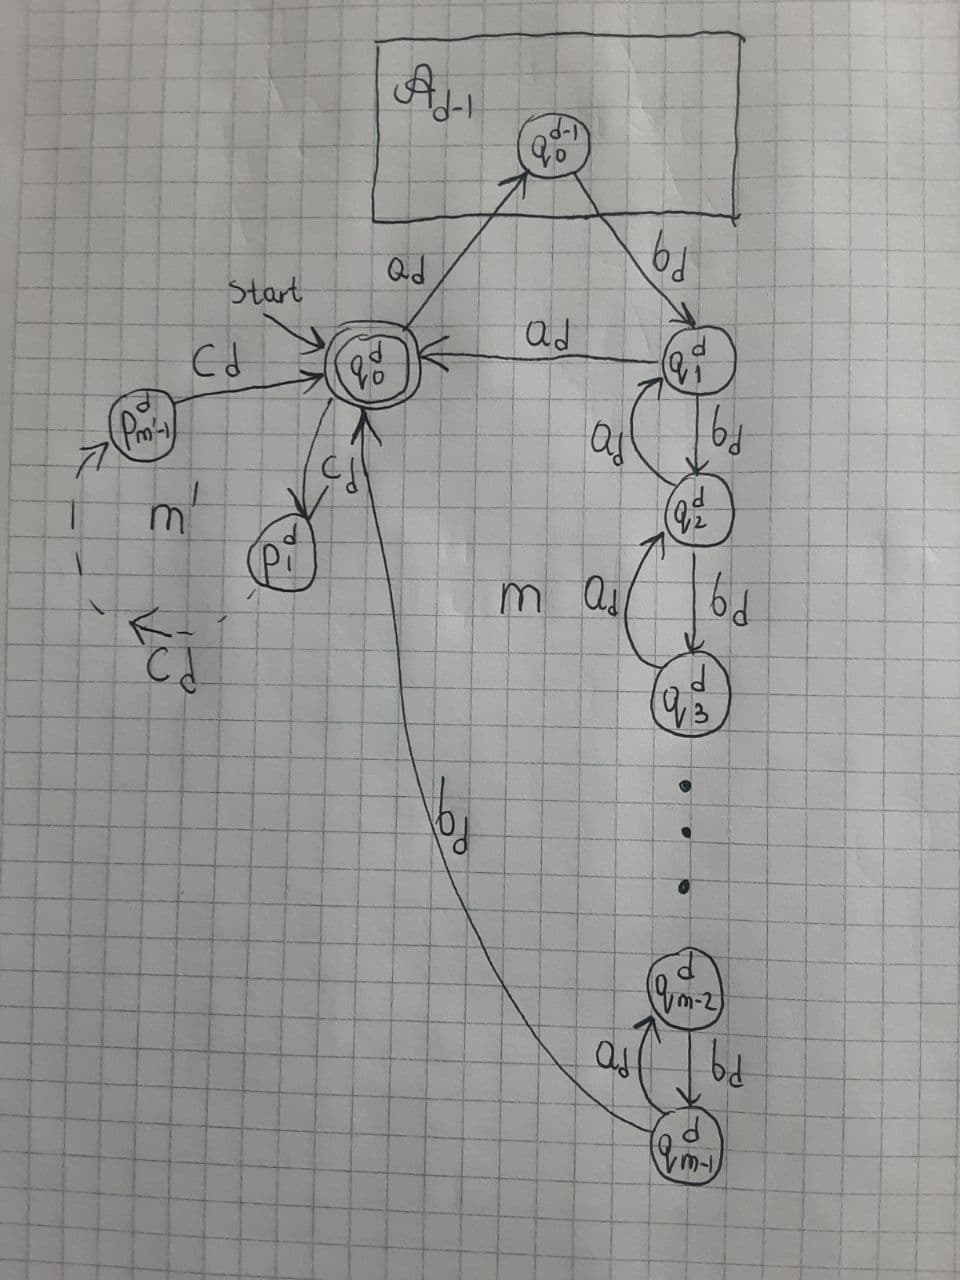
\includegraphics[width=.8\linewidth]{example_gen.jpg}
  \captionof{figure}{Обобщенный автомат $\mathcal{A}_{d}$}
  \label{dimautomata:generalized}
\end{minipage}%
\begin{minipage}{.5\textwidth}
  \centering
  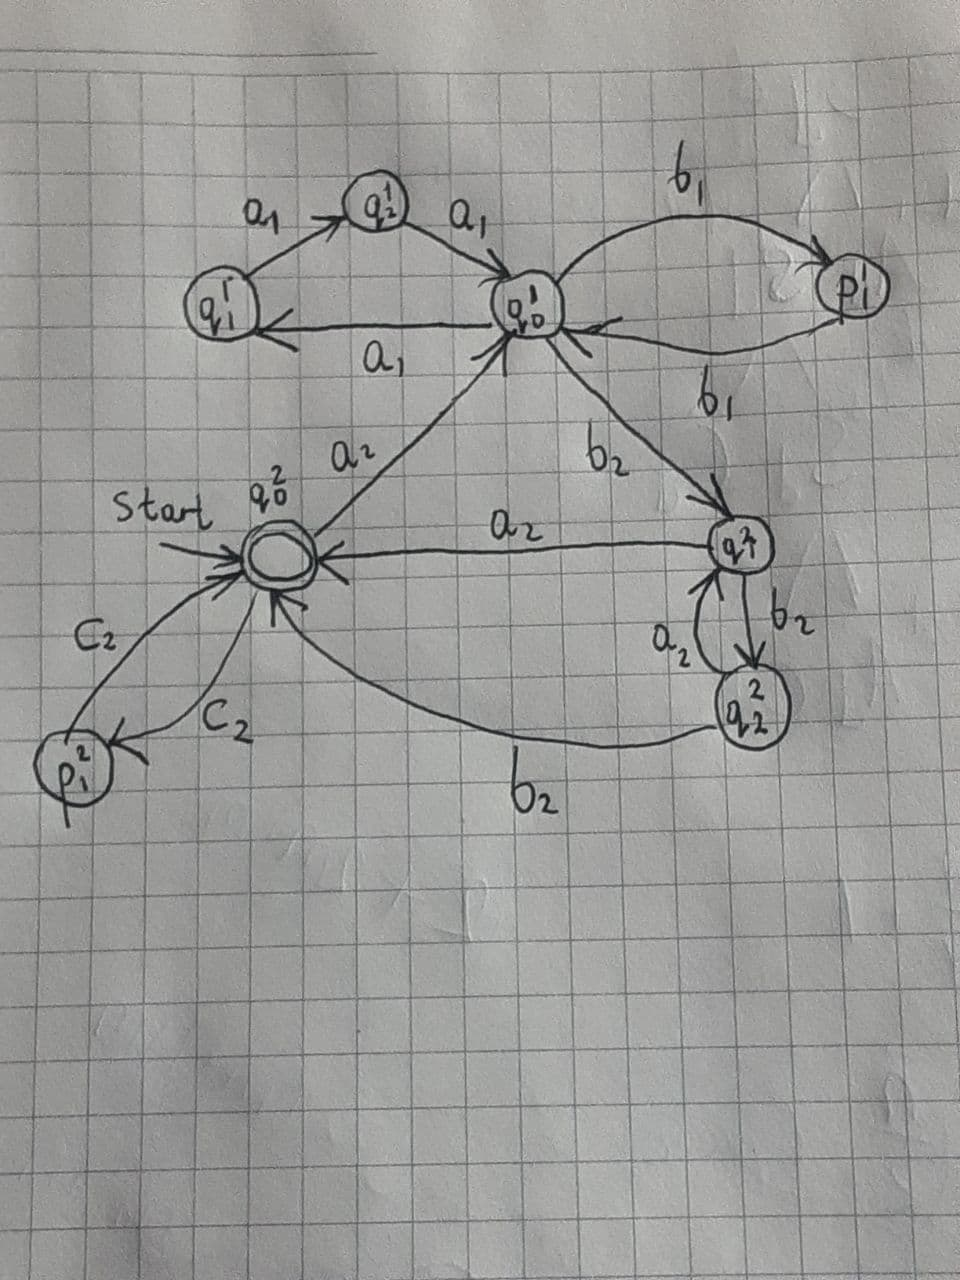
\includegraphics[width=.8\linewidth]{example2.jpg}
  \captionof{figure}{Автомат $\mathcal{A}_{2}$ c $n=8$ и $m = 3, m' = 2$}
  \label{dimautomata:2}
\end{minipage}
\end{figure}

\textit{Построение NFA $\mathcal{A}_{d} = (Q_d,\Sigma_d ,\delta_d ,q^{d}_{0},F_d$)} на $n$ вершинах. Без потери общности предположим, что $n$ делится на $4$.
Пусть число состояний $n'$ у автомата $\mathcal{A}_{d-1}= (Q_{d-1},\Sigma_{d-1} ,\delta_{d-1} ,q^{d-1}_{0},\{q^{d-1}_{0}\})$ равняется $n/2$. По индукционному предположению такой автомат существует. Зафиксируем два взаимно простых числа $m$ и $m'$ как $n/4+1$ и $n/4$ соответственно.
Тогда NFA $\mathcal{A}_{d}$ задается следующим образом:
\begin{itemize}
\item $\Sigma_{d} = \Sigma_{d-1} \cup \{a_d, b_d, c_d\}$
\item $\delta_{d} = \delta_{d-1} \cup \{
\\(q^{d}_{0}, a_d) \rightarrow q^{d-1}_{0},
\\(q^{d-1}_{0}, b_d) \rightarrow q^{d}_{1},
\\(q^{d}_{i}, b_d) \rightarrow q^{d}_{i+1}, 1 \le i \le m-1,
\\(q^{d}_{i}, a_d) \rightarrow q^{d}_{i-1}, 1 \le i \le m-1,
\\(q^{d}_{m-1}, b_d) \rightarrow q^{d}_{0},
\\(q^{d}_{0}, c_d) \rightarrow p^{d}_{1},
\\(p^{d}_{i}, c_d) \rightarrow p^{d}_{i+1}, 1 \le i \le m'-1,
\\(p^{d}_{m'-1}, c_d) \rightarrow q^{d}_{0}\}$
\item $F_d = \{q^{d}_{0}\}$
\item $Q_d = Q_{d-1} \cup \{ q^d_{0}, ..., q^d_{m-1}, p^d_{0}, ..., p^d_{m'-1}\}$
\end{itemize}
Общий вид автомата $\mathcal{A}_{d}$ показан на рисунке~\ref{dimautomata:generalized}.


Оценим длину кратчайшей строки из $L(G_d) \cap L(\mathcal{A}_{d})$. Зафиксируем кратчайшие строки $w_i = l(q^{d}_{i-1}\pi_iq^d_i)$ для $1 \le i \le m-1$ и $w_m = l(q^{d}_{m-1}\pi_mq^d_0)$, обладающие следующими свойствами:
\begin{enumerate}
\item $w_i \in L(A_d)$, где $0 \le i \le m$ и $L(A_d)$ --- язык, порождаемый нетерминалом $A_d \in N_d$, взятым в качестве стартового
\item $w_i = a_d w_{i-1} b_d$, a $w_0 = w_0^{d-1}$
\item Последовательность путей $\pi_1 \pi_2 ... \pi_m$ образует цикл из $q^d_0$ в $q^d_0$.
\end{enumerate}
Учитывая свойства выше, и правила грамматики $G_d$ $S_d \rightarrow A_dS_dc_d\vert A_dc_d$, кратчайшая строка $w_0^{d} \in L(G_d) \cap L(\mathcal{A}_{d})$ имеет вид:
$$w_0^{d} = ({\prod_{i=1}^m w_i})^{m'}{c}_d^{mm'}$$
Тогда длина $w_0^{d}$ может быть вычислена как:
$$|w_0^{d}| = ({\sum_{i=1}^m |w_i|})m' + mm' = (\sum_{i=1}^m (|w_0^{d-1}| + 2i))m' + mm'  = 
(\sum_{i=1}^m |w_0^{d-1}| + \sum_{i=1}^m 2i)m' + mm' = $$
$$ =  |w_0^{d-1}| m m' + m^2m' + mm' 
$$
Так как в автомате NFA $\mathcal{A}_{d-1}$ $n/2$ состояний, то по индукционному предположению $|w_0^{d-1}| =O( (n/2)^{2d - 2})$. Учитывая, что $m = n/4 +1$, $m' = n/4$ получаем следующее:
$$\rho_{L(G_d)} \ge |w_0^{d}| = O((n/2)^{2d - 2}) (n/4 + 1) n/4 + (n/4 + 1)^2 n/4  + (n/4 + 1) n/4 =$$ $$= O((n/2)^{2d - 2}) n^2/16 = O(n^{2d}).$$


\end{proof}
\end{theorem}
\begin{example}{}
На рисунке~\ref{dimautomata:2} изображен автомат $\mathcal{A}_{2}$ c $n = 8$ и $m = 3, m' = 2$, правила грамматики $G_2$ : $\{  S_2 \rightarrow A_2S_2c_2\vert A_2c_2; A_2 \rightarrow a_2A_2b_2 \vert  a_2S_1b_2; S_1 \rightarrow a_1S_1b_1 \vert a_1b_1\}$.
\end{example}



\begin{subsection}{The rational indices of some subclasses of languages of bounded dimension}  

\paragraph{Superlinear languages.} 
A context-free grammar $G = (\Sigma, N, P, S)$ is \textit{superlinear} \cite{superlinear} if all productions of $P$ satisfy these conditions:
\begin{enumerate}
\item there is a subset $N_L \subseteq N$ such that every $A \in N_L$ has only linear productions $A\rightarrow aB$ or $A\rightarrow Ba$, where $B \in N_L$ and $a \in \Sigma$.
\item if $A \in N \setminus N_L$, then $A$ can have non-linear productions of the form $A \rightarrow BC$ where $B\in N_L$ and $C \in N$, or linear productions of the form $A\rightarrow \alpha B$ $\vert$ $B \alpha$ $\vert$ $\alpha$ for $B \in N_L$, $\alpha \in \Sigma^*$.
\end{enumerate}
A language is \textit{superlinear} if it is generated by some superlinear grammar. 
\begin{theorem} Let $G$ be a superlinear grammar. Then $\rho_{L(G)}$ is in $O(n^4)$.
\end{theorem}
\begin{proof}
From the definition of superlinear grammar $G$ it is observable that its parse trees have dimension at most 2. From 
Theorem~\ref{oscbnddim}, if dimensions of all parse trees are bounded by some $k$ then the rational index $\rho_{L(G)}$ of such language is in $O(n^4)$.
\end{proof}
\end{subsection}
\paragraph{Ultralinear languages.} A context-free grammar $G = (\Sigma, N, P, S)$ is \textit{ultrealinear} if there exists a partition $\{N_0, N_1, ..., N_k\}$ of $N$ such that $S \in N_k$ and if $A \in N_i$, where $0 \le i \le k$, then $(A \rightarrow \alpha) \in P$ implies $\alpha \in \Sigma^*N_i\Sigma^*$ or $\alpha \in {(\Sigma \cup N_0 \cup ... \cup N_{i-1})}^*$. Such a partition is called an \textit{ultralinear decomposition}. A language is \textit{ultralinear} if it is generated by some ultralinear grammar. 


The ultralinear languages were originally defined by Ginsburg and Spanier \cite{Ginsburg1966FiniteTurnPA} as languages recognizable by finite-turn pushdown PDAs (a finite-turn PDA is a PDA with a fixed constant bound on the number of switches between push and pop operations in accepting computation paths). 

Every ultralinear language is generated by an ultralinear grammar in \textit{reduced form} \cite{WORKMAN1976188}.
\begin{definition}[The reduced form of ultralinear grammar]
An ultralinear grammar $G = (\Sigma, N, P, S)$ is in \textit{reduced form} if its ultralinear decomposition $\{N_0, N_1, ..., N_k\}$ is in the following form:
\begin{enumerate}
\item $N_k=\{S\}$ and $S$ does not appear in the right part of any production rule
\item if $(A \rightarrow \alpha) \in P \setminus \{S \rightarrow \varepsilon\}$ and $A \in N_i$, $0 \le i \le k$, then $\alpha \in (\Sigma \cup N_i\Sigma \cup \Sigma N_i \cup N_jN_{j'})$, where $j, j' < i$.
\end{enumerate}
\end{definition}
\begin {theorem}
Let $G = (\Sigma, N, P, S)$ be an ultralinear grammar with the ultralinear decomposition $\{N_0, N_1, ..., N_k\}$. Then $\rho_{L(G)}$ is in $O(n^{2k})$.
\end{theorem}
\begin{proof}
Recall that by definition dimension of a parse tree is the height of its largest perfect subtree. Consider the maximum possible size of a perfect subtree which occurs in the parse tree in ultralinear grammar in reduced form. It is easy to see that the rules of the form $A \rightarrow BC$, where $A \in N_i, B, C \in N_{i-1}$ should be used as often as possible to construct the largest binary subtree. Therefore, if grammar has the subset of rules of the form $\{S \rightarrow AB, A \rightarrow A_1A_2, B \rightarrow B_1B_2, A_1\rightarrow A_3A_4, ..., A_i \rightarrow A_{i+2}, A_{i+3}, ...\}$, where $A, B \in N_{k-1}, A_1, A_2, B_1, B_2 \in N_{k-2}, A_3, A_4, ... \in N_{k-3}, ... , A_{i+2}, A_{i+3}, ... \in N_0$, the perfect binary subtree obtained with these rules will be of height not greater than $k$, so the maximum dimension of the parse tree in a ultralinear grammar in reduced form is $k$. By Theorem~\ref{oscbnddim}  $\rho_{L(G)}$ is in $O(n^{2k})$.
\end{proof}


\section{Conclusions and open problems}
\label{sec:conc}

We have proved that bounded-oscillation languages
have polynomial rational index.
This means that the CFL-reachability problem and Datalog query evalution for these languages is in NC.
This class is a natural generalization of linear languages,
and might be the largest class of queries among such generalizations
that is known to be in NC.


There is a family of languages which has polynomial rational index,
but is incomparable with the linear languages:
\emph{the one-counter languages}.
Moreover, it is not comparable with the bounded-oscillation languages:
for example, the Dyck language $D_1$ is a one-counter language,
but not a bounded-oscillation language for any $k$.
Could this class be generalized in the same manner as linear languages
with respect to the polynomiality of the rational index?
One can consider the Polynomial Stack Lemma by Afrati et al.~\cite{ChainQ},
where some restriction on the PDA stack contents are given,
or investigate the properties of the substitution closure of the one-counter languages,
which is known to have polynomial rational index \cite{RatBasic}. 


%%For cite command type as \cite{1}; \cite{3,6} and \cite{2,4,6}.
%%For refcite command type as Refs.~[\refcite{1}];
%%[\refcite{1},\refcite{3}] and [\refcite{1}--\refcite{4}].


\begin{comment}
\section*{Acknowledgments}
This research was supported by the Russian Science Foundation, grant \textnumero 18-11-00100.
\end{comment}


\bibliographystyle{plain}
\bibliography{paper}
\end{document}